\lecture{8}{21. Oktober 2024}{Differentialregning i flere variable}
\begin{eks}[Overfladeareal af menneske]
  Et eksempel på en funktion af flere variable er følgende approksimation af overfladearealet af et menneske, $A(h, v)$, givet en højde $h$ og en vægt $m$
  \[
  A(h,v) = 0,024h^{0,3964}v^{0,5378}
  .\]
  Denne funktion kan bl.a. benyttes til at finde den forventede stigning i overfladeareal givet en vægtøgning eller en vækst i højde.
\end{eks}
En funktion af 2 variable kan kun plottes i 3-D idet denne indeholder tre variable $(x, y, f(x, y)$. En funktion af 3 variable ville kræve et 4-D rum for at kunne plottes.

Ved at "fastgøre" forskellige variable kan plottet dog vises med færre dimensioner end ellers påkrævet. 

\begin{figure} [ht]
  \centering
  \caption{Plots af $f(x,y) = x^2 + y^2$ med forskellige `faste' variable}
  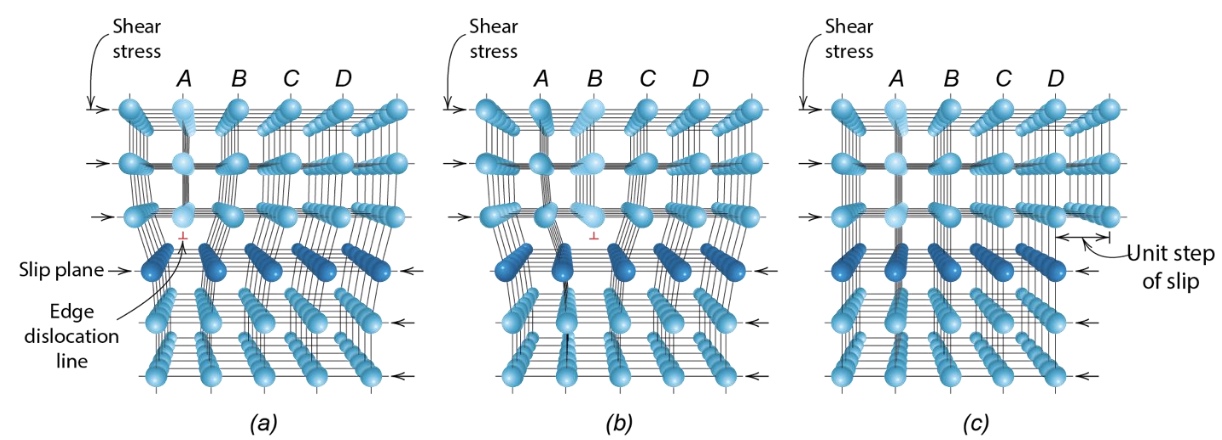
\includegraphics[width=0.8\linewidth]{./figures/f8_1.png}
  \label{fig:f8_1}
\end{figure}

På \autoref{fig:f8_1} ses den samme funktion, men hvor forskellige variable `fastholdes'.

En række ``standardfunktioner'' af flere variable eksisterer
\begin{itemize}
  \item Paraboloide
    \[ 
    z = x^2 + y^2
    .\]
  \item Ellipsoide
    \[ 
    \frac{x^2}{a^2} + \frac{y^2}{b^2} + \frac{z^2}{c^2} = 1
    .\]
  \item Hyperbolsk paraboloide (saddel)
    \[ 
    z = x^2 - y^2
    .\]
  \item Hyperboloide af to `sheets' 
    \[ 
    -x^2-y^2+z^2 = 1
    .\]
\end{itemize}

\section{Partielt afledede (Eng: \textit{Partial Derivatives})}
For at kunne lave differentialregning på funktioner med flere variable beskæftiger vi os med partielt afledede, hvor den ene (eller en række af) variablene fastholdes således at der kan differentieres for 1 variabel. Den partielt afledede af f ift. x skrives som
\[ 
\frac{\partial f}{\partial x}
.\]
Dette udtryk tilsvarer funktionen, $f$'s, vækstrate i retning af $x$. 

\begin{definition}[Definition af den partielt afledede]
  Mere specifikt har vi at den partielt afledede til $f(x, y)$ mht. $x$ i punktet $(x_0, y_0)$ er
  \[ 
  \frac{\partial f}{\partial x}(x_0, y_0) = \frac{\mathrm{d}}{\mathrm{d}x} f(x, y) |_{x = x_0}
  .\]
  Bemærk at notationen $f_x$ også benyttes for ovenstående.

  Det samme gør sig i øvrigt gældende langs $y$-aksen, $z$-aksen eller hvilken som helst anden akse.
\end{definition}

\begin{eks}[Partielt afledede i to retninger]
  Lad $f(x,y) = x^2 + 3xy + y -1$. Find $\frac{\partial f}{\partial x}$ og $\frac{\partial f}{\partial y}$ i punktet $(4,-5)$. 
  
  For at finde $\frac{\partial f}{\partial x}$ differentierer vi først ift. x så vi får at
  \[ 
  \frac{\partial f}{\partial x} = 2x + 3y
  ,\]
  og dermed har vi at
  \[ 
  \frac{\partial f}{\partial x}(4, -5) = 2\cdot4 + 3\cdot-5 = -7
  .\]
  
  Det samme gøres langs y-aksen hvor vi får at
  \[ 
  \frac{\partial f}{\partial y} = 3x+1
  ,\]
  og dermed har vi at
  \[ 
  \frac{\partial f}{\partial y}(4,-5) = 4\cdot3 + 1 = 13
  .\]
\end{eks}

\begin{eks}[En mere kompliceret funktion]
  Lad 
  \[ 
  f(x,y) = \frac{2y}{y + \cos(x)}
  .\]
  Find $f_x$ og $f_y$.

  Vi finder først $f_x$ som
  \[ 
  f_x = \frac{\partial f}{\partial x} = \frac{2y \sin(x)}{(y + \cos(x))^2}
  .\]
  
  Slutteligt findes $f_y$ som
  \[ 
  f_y = \frac{\partial f}{\partial y} = \frac{2 \cos(x)}{(y + \cos(x))^2}
  .\]
\end{eks}

\begin{eks}[Funktioner af mere end to variable]
  Lad
  \[ 
  f(x,y,z) = x \sin(y+3z)
  .\]
  Find $f_z$.
  Vi finder den afledte med hensyn til $z$, $f_z$ som
  \[ 
  \frac{\partial f}{\partial z} = 3x \cos(y + 3z)
  .\]
\end{eks}

\section{2. Ordens partielle afledede}
For 2. ordens partielle afledede introduceres følgende notation for den afledte af $f$ mht. $y$ og derefter mht. $x$
\[ 
f_{yx} = \frac{\partial^2 f}{\partial x \partial y} \coloneq \frac{\partial }{\partial x} \frac{\partial f}{\partial y}
.\]
Og tilsvarende for den afledte mht. $x$ 2 gange
\[ 
f_{x x} = \frac{\partial^2 f}{\partial^2 x} \coloneq \frac{\partial }{\partial x} \frac{\partial f}{\partial x}
.\]
De fire 2. ordens afledte af funktionen med to variable $f(x, y)$ er
\begin{enumerate}
  \item $f_{x x}$
  \item $f_{y y}$
  \item $f_{x y}$
  \item $f_{yx}$
\end{enumerate}

\begin{eks}
  Lad
  \[ 
  f(x,y) = x \cos(y) + ye^{x}
  .\]
  Find de fire anden ordens afledte.
  
  Vi finder den partielt afledte mht. $x$ som
  \[ 
  \frac{\partial f}{\partial x} = \cos(y) + ye^{x}
  .\]

  Og den afledte mht. $y$ som
  \[ 
  \frac{\partial f}{\partial y} = -x\sin(y) + e^{x}
  .\]
  De fire 2. ordens afledte findes derefter som
  \begin{align*}
    \frac{\partial^2 f}{\partial^2 x} &= \frac{\partial }{\partial x} \cos(y) + ye^{x} = ye^{x}  \\
    \frac{\partial^2 f}{\partial^2 y} &= \frac{\partial }{\partial y} -x \sin(y) + e^{x} = -x \cos(y)  \\
    \frac{\partial^2 f}{\partial y \partial x} &= \frac{\partial }{\partial y} \cos(y) + ye^{x} = -\sin(y) + e^{x}  \\
    \frac{\partial^2 f}{\partial x \partial y} &= \frac{\partial}{\partial x} -x \sin(y) + e^{x} = -\sin(y) + e^{x} \\
  .\end{align*}
\end{eks}

\section{Maksimum og minimum}
\begin{sæt}[Definition af relativt maksimum og minimum] \label{sæt:1}
  \textbf{Relativt maksimum:} Et punkt $(a,b)$ er et relativt maksimum hvis $f(a,b) \geq f(x,y)$ for alle $(x,y)$ i en lille omegn af $(a,b)$.

  \textbf{Relativt minimum:} Tilsvarende gælder at hvis der for et punkt $(a,b)$ gælder at $f(a,b) \leq f(x,y)$ for alle $(x,y)$ i en lille omegn af $(a,b)$ så er $(a,b)$ et relativt minimum.
\end{sæt}

Af sætning \autoref{sæt:1}.1 har vi at et punkt $(a,b)$ er et kritisk punkt for $f$ hvis $f_x(a,b) = f_y(a,b) = 0$. 

\begin{eks}
  Find de kritiske punkter for
  \[ 
  f(x,y) = 4x^3 + 3xy + 4y^3
  .\]
  Først findes $\frac{\partial f}{\partial x}$ som
  \[ 
  f_x = 12x^2 + 3y
  .\]
  Og dernæst findes $\frac{\partial f}{\partial y}$ som
  \[ 
  f_y = 3x + 12y^2
  .\]
  Vi har dermed 2 linginger med 2 ubekendte
  \begin{align*}
    0 &= 12x^2 + 3y & 0 &= 3x + 12y^2 \\
    y &= -4x^2 & 0 &= 3x + 12(-4x^2)^2 = 3x \left( 1 + 64x^3 \right) \\
    y &= -4(-\frac{1}{4})^2 = -\frac{1}{4} & x &= -\frac{1}{4}
  \end{align*}
  Derudover er $(0,0)$ et kritisk punkt så de to kritiske punkter er $(0,0)$ og $(-\frac{1}{4}, -\frac{1}{4})$
\end{eks}

Bemærk at et relativt maksimum eller minimum medfører et kritisk punkt, men den modsatte implikation gælder ikke. Et kritisk punkt kan godt hverken være et maksimum eller minimum, hvilket er tilfældet med \textit{saddelpunkter}.

\subsection{2. ordens test for maksimum/minimum eller saddelpunkt}
Hvis du ved at $(a,b)$ er et kritisk punkt kan du finde ud af om det er et maksimum, minimum eller et saddelpunkt ved at beregne diskriminanten $D$ givet ved
\[ 
D = f_{x x}(a,b)f_{yy}(a,b) - f_{xy}(a,b)^2
.\]
Der gælder derefter at
\begin{itemize}
  \item Hvis $D<0$ er $(a,b)$ et saddelpunkt
  \item Hvis $D = 0$ har du ingen information
  \item Hvis $D>0$ og $f_{x x}(a,b)<0$ er $(a,b)$ et relativt maksimum
  \item Hvis $D>0$ og $f_{x x}(a,b)>0$ er $(a,b)$ et relativt minmum
\end{itemize}

